\subsubsection{Hipótesis}

Para este filtro esperamos observar, como primer analisis, que las implementaciones tengan un crecimiento estable a medida que van creciendo una misma cantidad de píxeles pero con diferente organización.

Como segundo analisis, creemos que las implementaciones realizadas en ASM sean mas eficientes que la realizada en C, sin importar el tamaño de la entrada, ya que la implementación en C procesa los pixeles de manera independiente y ambas implementaciones en ASM utilizan operaciones del formato \textbf{SSE} y procesan más píxeles al mismo tiempo.

Entre las dos implementaciones de ASM, esperamos que la implementación ASM 2 (\textbf{sepia_asm2.asm}) sea levemente más eficiente frente a la implementación ASM 1 (\textbf{sepia_asm.asm}) ya que posee una operación menos para realizar los calculos sobre los pixeles y no posee una operación de división (\textbf{divps}), que si posee ASM 1.

\subsubsection{Resultados Obtenidos - Primer Analisis}

Los siguientes graficos presentan los resultados obtenidos de nuestro primer analisis en donde realizamos la comparación de cada una de las implementaciones consigo misma con el fin de observar si se generan resultados diferentes para una misma cantidad de píxeles pero con diferente organización.

\begin{figure}[h!]
	\centering
		\begin{tabular}{cc}
		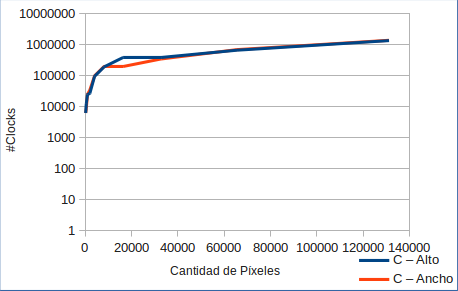
\includegraphics[width=250px]{imgs/sepia-c-analisis1.png} &
		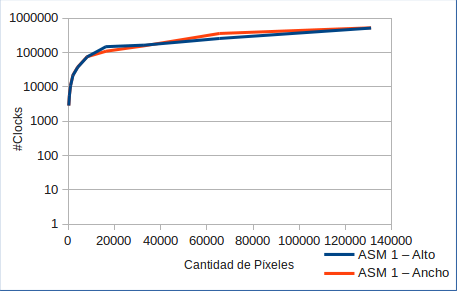
\includegraphics[width=250px]{imgs/sepia-asm1-analisis1.png} \\
		\end{tabular}
		\begin{tabular}{c}
		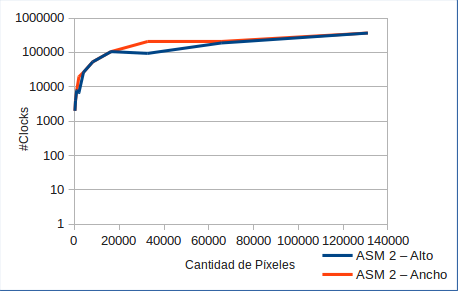
\includegraphics[width=250px]{imgs/sepia-asm2-analisis1.png} \\
		\end{tabular}
\end{figure}

Podemos observar que las curvas de crecimiento de nuestras tres implementaciones del filtro tienden a tener un mismo comportamiento a media que la cantidad de pixeles va en aumento, lo que afirma nuestra hipótesis sobre este primer analisis. Por otro lado, también puede observarse que para tamaños de entrada de entre 20000 y 40000 píxeles las tres implementaciones generar una diferencia, en alguno mas sutil como en ASM 1 y en otro mas marcada como en la de ASM 2. Este comportamiento inesperado sería interesante estudiarlo posteriormente.

\subsubsection{Resultados Obtenidos - Segundo Analisis}

Los siguientes graficos presentan los resultados obtenidos de nuestro segundo analisis en donde realizamos la comparación de performance de cada una de las implementaciones con las demás.

\begin{figure}[h!]
	\centering
	\begin{tabular}{ll}
		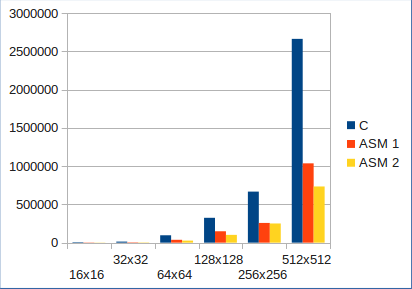
\includegraphics[width=250px]{imgs/sepia-analisis2-1.png} & 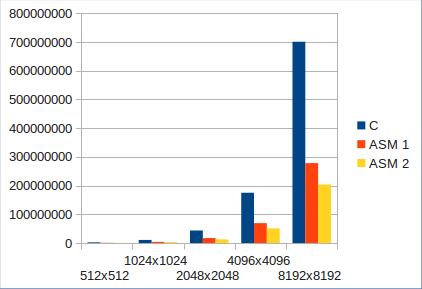
\includegraphics[width=250px]{imgs/sepia-analisis2-2.png} \\
		\vspace{1em}
	\end{tabular}
\end{figure}

Como podemos observar, la implementación en C (con O3) resultó ser mucho menos eficiente que sus contrapartes de ASM (que obtubieron ganancias del 70\% y 80\% con respecto a la implementación en C), a medida que la imagen va creciendo, esto afirma nuestra primera parte de la hipotesis. Por otro lado, entre los algoritmos ASM 1 y ASM 2 pudimos observar que se obtuvo una mas pequeña mejora en performance del ASM 2 sobre ASM 1. Esto afirma nuestra segunda parte de la hipotesis, las operaciones de división y sumas que posée la implementación ASM 1 son mucho mas costosas que las multiplicaciones que posée la implementación ASM 2 y esto se refleja en la diferencia de 0.36x superior en el tiempo de ejecución de ASM 1 con su contraparte ASM 2.

\begin{table}[!htbp]
	\centering
	\footnotesize
	\begin{tabular}{| c | c | c | c |}
		\hline
Pixels &ASM 2 & ASM 1 & C (O3) \\ \hline
16x16 & 1996 & 2862 & 6278 \\ \hline
32x32  &4232  & 4869 & 13580 \\ \hline
64x64  & 26383 & 37273 & 96682 \\ \hline
128x128 & 101613 & 148681 & 324678 \\ \hline
256x256  & 250612  & 257940 & 667089 \\ \hline
512x512   & 733971 & 1036902 & 2664477 \\ \hline
1024x1024 & 3161181 & 4314780 & 10863381 \\ \hline
2048x2048  & 12802011 & 17375403 & 43898460 \\ \hline
4096x4096 & 51152475 & 69574692 & 175335426 \\ \hline
8192x8192 & 204137541 & 278365320 & 700733874 \\ \hline
Tiempo en X& 1x & 1.36x & 3.43x \\ \hline
Ganancia vs C & 70.86\% & 60.29\%	& 100.00\% \\ \hline

	\end{tabular}
\end{table}